\section{Methods}

\subsection{Dataset}
\subsubsection{Ophav}
Hvor har vi dette datasæt fra, og hvem har lavet det?

\subsubsection{Features}
Skrive noget om hvad vores datasæt er og hvordan det er sat op. Dvs. hvilke egenskaber er der, hvordan er de encoded (one-hot vs. binært (solvent)) og hvorvidt vi bruger dem til noget. Fortæl også om at strukturerne her er encoded som de 8 substrukturer og ikke de 3 grupperinger af strukturer.

\subsubsection{Opdeling i træning, test og validering}
Fortæl om at vi har rigtigt meget træningsdata og hhv. 255 og 236 værdier i test og validering. Vi træner og backpropagerer over træningssættet, holder øje med valideringssættet (og træffer vores beslutninger ud fra det) og udsætter kun modellen for testsættet til sidst.

\subsection{Tools}
\subsubsection{Model}
Being that we are training a convolutional neural network, in particular two sets of functions are important, namely activation and loss functions.

The activation functions we opted to use in this project were the rectifier, softmax and sigmoid functions respectively, whereas we use the Cross Entropy loss in evaluating and training the network.
\paragraph{Rectifier}
Possibly the simplest of these activation functions is the rectifier, which when implemented in an artificial neural network is referred to as a \textit{rectified linear unit} (ReLU), which, in laymans terms, simply does not allow negative values, and replaces such values with zero.
\[
ReLU(x) = x^+ = max(0,x)
\]

\paragraph{Sigmoid function}
Sigmoid functions are a specific variant of logistic functions, and serve to map values in arbitrary ranges to values within a specific range, so that the mapped values over the original values form a sigmoid curve. The value of applying sigmoid functions to outputs from a neural network is that they then enable the model to map its output of arbitrarily big or small values to a probability (i.e. a value $0\leq x \leq 1$). In the present case, this becomes relevant when predicting relative and absolute solvent accessibilities.
\[
Sigmoid(x) = \frac{1}{1 + e^{-x}} = \frac{e^x}{e^x +1}
\]

\begin{figure}[h]
  \centering
  \frame{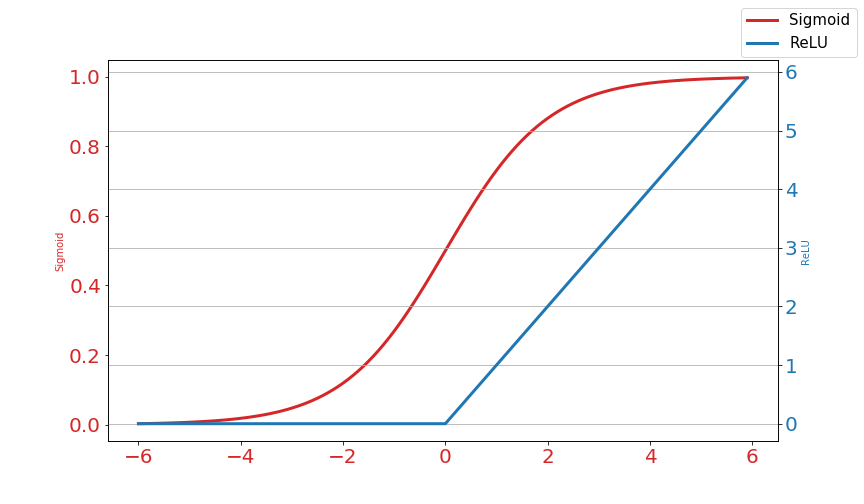
\includegraphics[width=\linewidth]{../graphs/activation}}
  \caption{The sigmoid and rectifier activation functions}
\end{figure}

\paragraph{Softmax}
The softmax function ($\sigma$) does very much the same as the sigmoid, only for a range of values. In other words, a set of non-normalized values (that is: of arbitrary length and spread) can via softmax be mapped to a probability distribution over that set. This means that all the values $x_i$ are in the range $0\leq x_i \leq 1$, and that they sum to 1.

This is especially relevant in cases where one is attempting to perform classification, such as which is the present case where we are training the model to predict amino acid secondary structures. 

Applying a softmax function on a dataset \textit{x} of \textit{j} elements would be as follows:
$$
\sigma(x_i) = \frac{e^{x_i}}{\sum_{j=1} e^{x_j}}
$$

\begin{figure}[h]
  \centering
  \frame{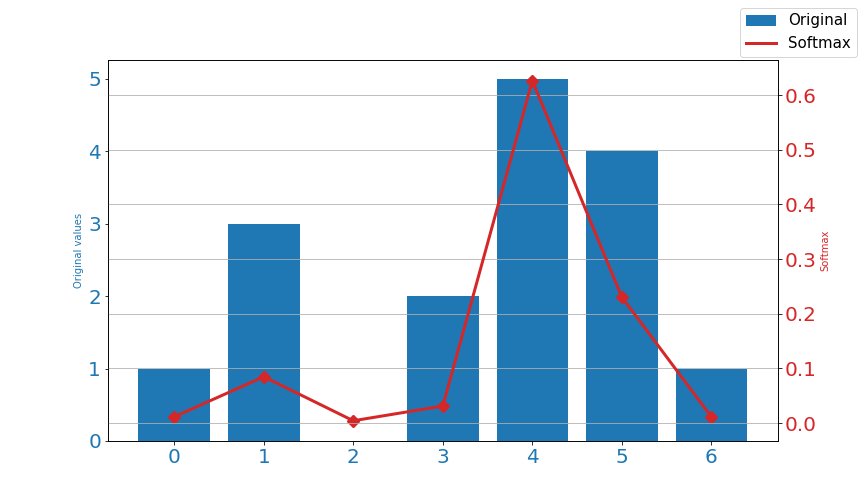
\includegraphics[width=\linewidth]{../graphs/softmax}}
  \caption{Example data softmaxed}
\end{figure}


\paragraph{Cross Entropy Loss}
Between two probability distributions each over the same set of outcomes there exists a certain cross entropy.
Thus, given two probability distributions \textit{m} and \textit{n} predicting the discrete outcome $\mathcal{Z}$, the formula for calculating the cross entropy is:
$$L ( m , n ) = - \sum _ { z \in \mathcal { Z } } m ( z ) \log n ( z )$$
A specific instance of the cross entropy loss is the \textit{binary cross entropy loss}, which is useful in cases where the possible outcome is binary (i.e. there are only two possible outcomes). In this case the formula becomes:\\
\[
\ell(m, n)=L=\left\{l_{1}, \ldots, l_{N}\right\}^{\top}
\]
where
\[ \quad l_{n}=-w_{n}\left[n_{n} \cdot \log m_{n}+\left(1-n_{n}\right) \cdot \log \left(1-m_{n}\right)\right]
\]
\\
Seing as the aim of this paper was to train our network to perform classifications first on amino acid secondary structures (of which there are eight) and then relative and absolute solvent accessibility (which are both encoded as either ones or zeros), we have used a Cross Entropy Loss function on the former and a Binary Cross Entropy Loss function on the two latter.


\subsubsection{Technological implementation details}
In training our network we utilized a machine learning framework for Python called \href{https://pytorch.org/}{PyTorch}, specifically optimized for building deep neural networks. \\
The PyTorch library is build upon the \href{http://torch.ch/}{Torch} library, originally a machine learning library and language based on the scripting language Lua.\\
The strength in using PyTorch stems from several aspects:
\paragraph{GPU support}
PyTorch provides a strong framework for performing calculations on a graphical processing unit rather than the computer's CPU. While GPUs are valued in video game circles, they are also enourmously useful for performing machine learning, since this is often tasks that involve a high number of calculations that can perfectly fine be performed in parallel. For this, a GPU is preferred over a CPU since they often have a much higher number of cores, and are thus better suited for parallel programming.
\paragraph{Tensors}
The main data structure used in the PyTorch framework is tensors. In this context, a tensor is to mean a multi-dimensional array much like the ones implemented in numpy, but with the option to place it on the GPU rather than the CPU.
\paragraph{Automatic differentiation}
In order to utilize the backpropagation that lets neural networks train and improve, the loss must be differentiated in regards to all of the weights and values in the model in order to calculate the gradients. This can be a cumbersome task when performed by hand, but PyTorch provides a powerful tool in for of the \texttt{autograd} and \texttt{optim} modules. The first of these modules keeps track of which computations were performed on which variables in order to arrive at the final value of a variable, so that it can be retraced backwards in the end to calculate gradients, while the latter automatically adjusts the weights and values in the model, according to the calculated gradient and a supplied learning rate.

These things combined indeed allow a training step for a neural network to be performed in as few steps as shown below:
\begin{lstlisting}
# Setup
LR = 0.0025              # learning rate
optimizer = torch.optim.Adam(cnn.parameters(), lr=LR)
loss_func = nn.CrossEntropyLoss()

# One training step
output = cnn(b_x)
loss = loss_func(output, b_y)
optimizer.zero_grad()
loss.backward()
optimizer.step()
\end{lstlisting}
In terms of performing the calculations, all of our training of the model was done on a Dell PC with a 7th gen 8-cores Intel Core i7 CPU, 16GB of RAM and a Nvidia GeForce GTX 1050TI GPU with 4GB of RAM and 768 cores running Linux.

\subsection{Predicting secondary structures alone}
Fortælle om hvordan vi byggede vores single-model (convolutionelle lag, ReLU, softmax, BCELoss, padding).

\subsubsection{Beregning af præcision}
Forklar at det vi tæller er antallet af korrekte forudsigelser over antal af faktiske aminosyrer. Gennemgå herunder matematikken i at vi kollapser fra one-hot til classification, og så kører vores mask-magi på det.

\subsection{Implementing multitask learning}
\subsubsection{Generelt om Multi-task learning}
Start med refleksioner over hvordan vi bruger shared-parameters i vores model, og forklar at vi stadig kører udelukkende konvolutionelle lag igennem modellen.
\subsubsection{Opbygningen af vores model}
Fortæl om opbygningen af vores model - dvs. at vi ReLU'er hele vejen igennem, undtagen sidste lag, og så hvordan vi splitter dataen ud for så at ReLU'e og softmax'e sekundærstrukturerne, medens at vi afrunder solvent-egenskaberne.

\subsubsection{Træning}
Fortæl hvordan vi udregner loss på vores model, dvs. at vi udregner tre losses; sekundærstruktur, relativ solvency og absolut solvency. Vi bruger BCE på dem alle sammen, så redegør hvorfor vi godt kan det på solvent også.

\subsubsection{Beregning af præcision}
Forklar hvordan vi til strukturerne bruger samme beregning som ovenfor, mens vi gør næsten det samme for solvent egenskaberne (men hver for sig).

\subsection{Hyperparametre}
Fortæl at vi i projektet vil prøve at iterere over forskellige hhv. lagstørrelser, antal lag, kernelsizes, og learning rate.
Forklar at vi vil starte med at tage udgangspunkt i de værdier som Xi bruger, og så iterere lidt frem og tilbage over dem.





